$G$を非コンパクトな実半単純Lie群,$K$を$G$の極大コンパクト部分群で$G$のCartan対合$\Theta$に対して$K = \Theta K $なるものとする.$\ge = \ka \oplus \pe $を$\Theta$の微分$d\Theta$による$\ge$のCartan分解とするとき,$G/K$は$\pe$と$\pe \ni X\mapsto e^{X}K\in G/K $により微分同相である.

$H$を$G$の非コンパクトな閉部分群で,$H = \Theta H$を満たすものとし,$\per{\ha}\defeq \{W\in \ge\mid B(W, \ha) = \{0\} \} $とするとき,$G/K$と$\pe$の微分同相についてより強い次の構造定理が知られている.

\begin{thm*}(\cite[Lemma~6.1]{kob89})\label{thm:kob89-lem6.1}  
  $\pi\colon  (\ha\cap\pe)\oplus (\per{\ha}\cap \pe) \ni (Y, Z)\mapsto e^{Y}e^{Z}\cdot o_K \in G/K $は上への微分同相である.
\end{thm*}
この定理を用いて$X\in \pe$に対し,${(Y(X), Z(X))\defeq \inv{\pi}(e^X\cdot K)\in (\ha\cap\pe)\oplus (\per{\ha}\cap \pe)}$と定義する.

$G/K$に$\ge$のKilling形式$B$から定まるRiemann計量によってRiemann多様体の構造を定める.$G$の単位元の$G/K$での像$eK$を通る$G/K$の極大測地線は$B(X, X) = 1 $なる$X\in \pe$によって$e^{tX}K $,$t\in \real$と書ける.\Cref{thm:kob89-lem6.1}より任意の$t\in \real$に対して$e^{tX}K = e^{Y(tX)}e^{Z(tX)}K $である.

$G = \SU(1,1) $,$H = \SO(1,1) $とするとき,$t\in \real$に対し,$Y(tX) $は\Cref{fig:y-and-z}に図示するような幾何学的な意味を持つ.\Cref{fig:y-and-z}は{\Poincare}円板における測地線$e^{tX}K$ (赤色の斜め線) とその上の一点$e^{tX}K$から$eK$の$H$軌道 (中央の直線) に下ろした垂線の足 (緑の丸) が$e^{Y(tX)}K $である.
\begin{figure}[H]
  \centering
  %   \raggedleft
  %   \raggedrightp
  %   \includegraphics[scale=0.08]{graph/fig1.jpg}
  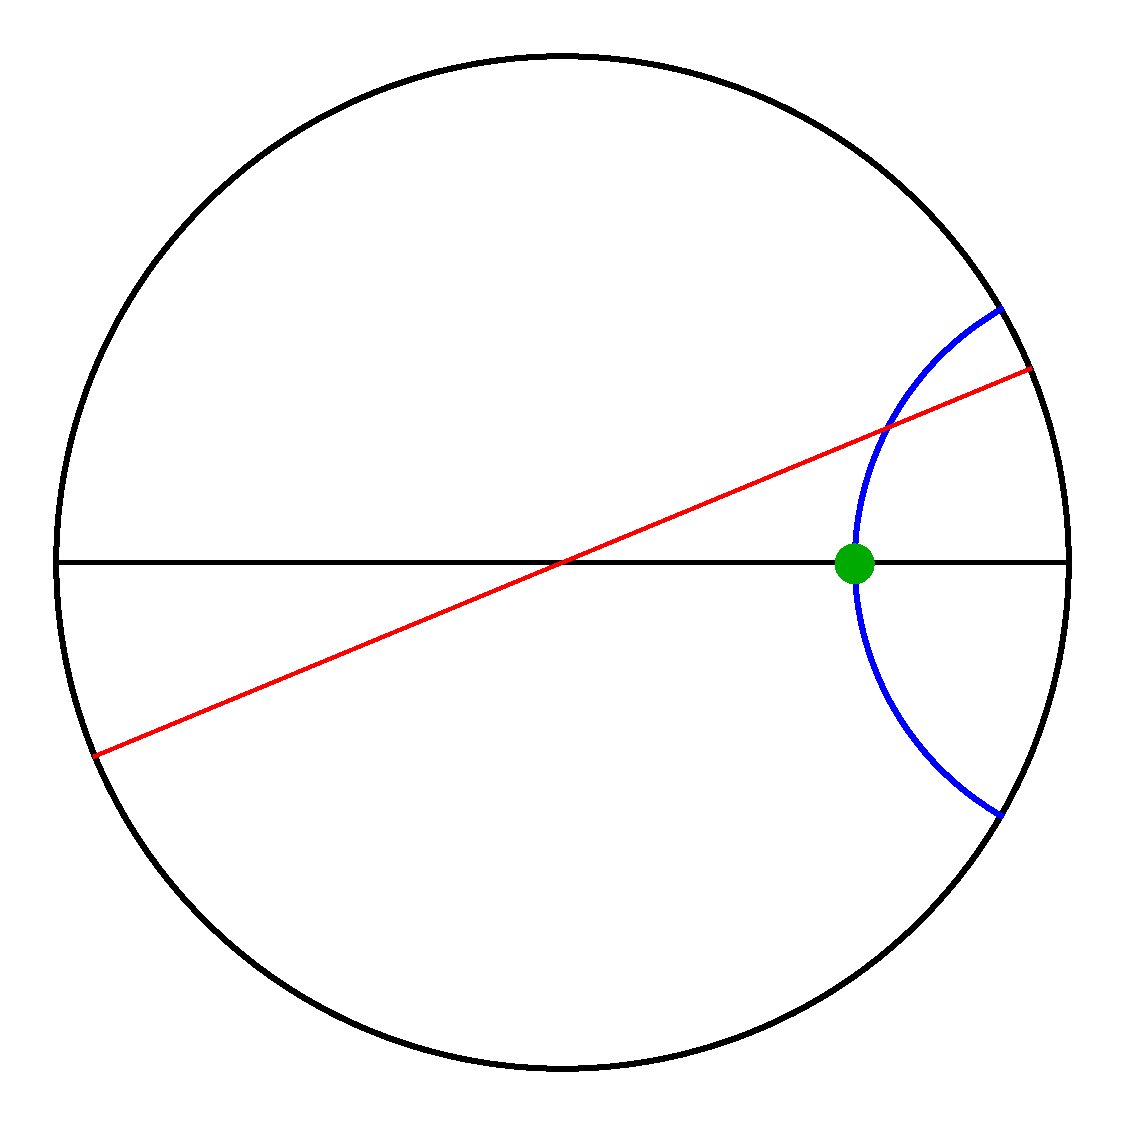
\includegraphics[scale=0.3]{../graph/y-and-z.pdf}
  \caption{{\Poincare}円板における$Y(tX) $の幾何学的意味}
  \label{fig:y-and-z}
\end{figure}

本論文では小林俊行氏による次の問題 (後述の\Cref{prob:1121}) について考察し,$G$が実階数1の実半単純Lie群の場合に肯定的な結果を得た.
\begin{prob*}
  $Y(\real X)$が$ \ha\cap \pe$の有界な部分集合であることと「$X\in \per{\ha}\cap\pe $もしくは『$ [X_1, X_2]\neq 0 $かつ$\ze_{\ze(\ha)}(X) = 0$であること』」は同値であるか?

  ただし$X = X_1 + X_2 $はベクトル空間としての分解$\pe =(\pe\cap \ha)\oplus(\pe\cap\per{\ha}) $に対応する$X\in \pe$の分解とする.
\end{prob*}

ここで$G$が実階数1のとき,「$X\in \per{\ha}\cap\pe $もしくは『$ [X_1, X_2]\neq 0 $かつ$\ze_{\ze(\ha)}(X) = 0$であること』」と$X\in \{0\}\cup\pe\setminus\ha $は同値である (後述する\Cref{lem:basic-prob}の3).
